\begin{figure}[h]
  \centering
  \begin{tabular}{ p{5cm} p{5cm} p{5cm} }
    \centering 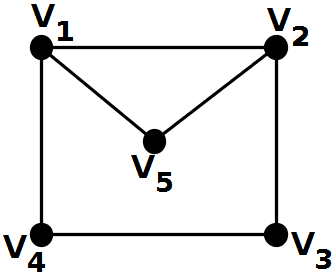
\includegraphics[width=3cm]{./img/envelope.png} & 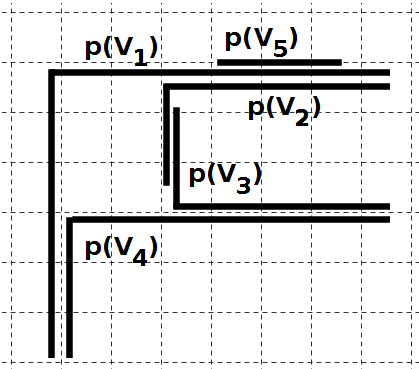
\includegraphics[width=4cm]{./img/envelopeHellyGradeTransparente.png} & 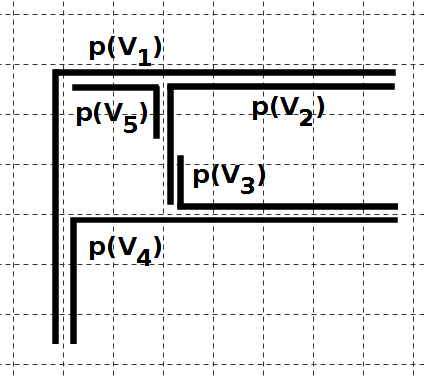
\includegraphics[width=4cm]{./img/envelopeNaoHellyGrade.png}
    \\
    \footnotesize \centering (a) A  graph with 5 vertices & \footnotesize(b) $B_1$-EPG representation that satisfies the Helly property & \footnotesize (c) $B_1$-EPG representation that does  not satisfy the Helly property  \\
% &&  \\ 

% \begin{tabular}[c]{@{}l@{}} 
% \hspace{3.3cm} 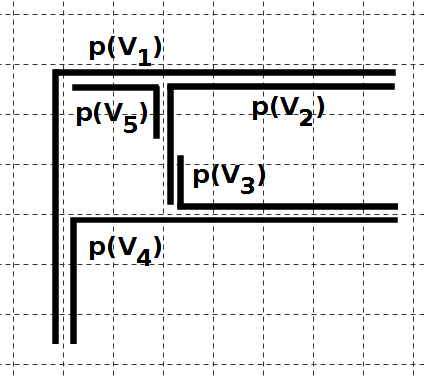
\includegraphics[width=4cm]{./img/envelopeNaoHellyGrade.png} %b1epgtriangulo
% \\
%  \hspace{3.3cm} \footnotesize (c) $B_1$-EPG representation that does\\ 
%  \hspace{3.3cm} \footnotesize not satisfy the Helly property
% \end{tabular}

% \centering &
% 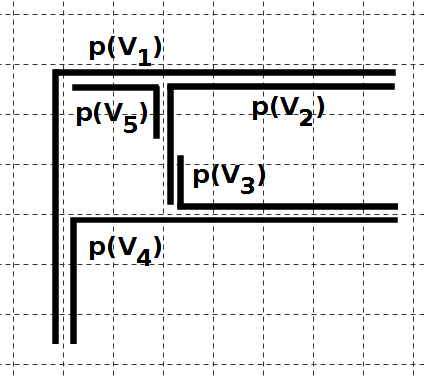
\includegraphics[width=5cm]{./img/envelopeNaoHellyGrade.png} %b1epgtriangulo
%       &
%  \\
%   \footnotesize \centering (c) $B_1$-EPG representation that not satisfies the Helly property &  &  \\
  \end{tabular}
\caption{A  graph with 5 vertices in (a) and some single bend representations: Helly in (b) and not Helly in (c)} \label{fig:envelopeRepresentacoes}
\end{figure}